% 18-09-2024

\chapter{Espacios Topológicos}

\begin{definicion}
    Un \textbf{espacio topológico} es una par $(X, \cc{T})$, donde $X \neq \emptyset$ es un conjunto y $\cc{T}\subset\cc{P}(X)$ es una familia de subconjuntos de $X$. Esta familia $\cc{T}$ tiene las siguientes propiedades:

    \begin{enumerate}
        \item[\objetivo{A1}] $\emptyset, X \in \cc{T}$.
        \item[\objetivo{A2}] Si $\{U_i\}_{i\in I} \subset \cc{T}$, entonces $\cuptext{i\in I} U_i \in \cc{T}$ (unión arbitraria\footnote{Puede ser finita o infinita, numerable o no numerable}).
        \item[\objetivo{A3}] Si $U_1, U_2 \in \cc{T}$, entonces $U_1 \cap U_2 \in \cc{T}$.
    \end{enumerate}

    A la familia $\cc{T}$ se le llama \textbf{topología} en el conjunto $X$. A los elementos de $\cc{T}$ se les llama \textbf{abiertos} en el espacio topológico $(X, \cc{T})$.
    \endsquare
\end{definicion}

\begin{observacion}
    De \apuntar{A3} podemos concretar que si $U_1, \dots, U_k \in \cc{T}$, entonces $\bigcap\limits_{i=1}^{k}U_i \in \cc{T}$, es decir, que la intersección finita de abiertos es abierto (se prueba con una inducción trivial).

    En general, si $\{U_i\}_{i=1}^{\infty}\in \cc{T}$, entonces $\bigcup\limits_{i=1}^{\infty}U_i$ no tiene por qué ser abierto.
    \endsquare
\end{observacion}

\begin{ejemplo}\ 
    \begin{itemize}
        \item \textbf{Topología trivial:} Sea $X \neq \emptyset$, $\cc{T}_t = \{\emptyset, X\} \Rightarrow (X, \cc{T}_t)$ es un e.t\footnote{A partir de ahora notaremos así a un espacio topológico}.
        \item \textbf{Topología discreta:} Sea $X \neq \emptyset$, $\cc{T}_{disc}= \cc{T}_{D} = \cc{P}(X) \Rightarrow (X, \cc{T}_D)$ es un e.t.
        \item \textbf{Topología del punto incluido:} Sea $X \neq \emptyset$, $x_0\in X$,
        
        $\cc{T}_{x_0} = \{\emptyset\}\cup \{U \subset X : x_0 \in U\} \Rightarrow (X, \cc{T}_{x_0})$ es un e.t.
        \item \textbf{Topología cofinita:} (o topología de los complementos finitos) Sea $X \neq \emptyset$,
        
        $\cc{T}_{CF} = \{\emptyset\}\cup\{U\subset X : X \setminus U \text{ es finito}\} \Rightarrow (X, \cc{T}_{CF})$ es un e.t. (por las leyes de Morgan)
        \begin{align*}
            X \setminus \left(\bigcup\limits_{i\in I}U_i\right) &= \bigcap\limits_{i\in I}(X \setminus U_i) \text{(intersección de finitos es finito)}\\
            X \setminus (U_1 \cap U_2) &= (X\setminus U_1) \cup (X \setminus U_2)\text{(unión de finitos es finito)}
        \end{align*}
        \item \textbf{Topología conumerable:} (o topología de los complementos numerables) Sea $X \neq \emptyset$, $\cc{T}_{CF} = \{\emptyset\}\cup\{U\subset X : X \setminus U \text{ es numerable}\} \Rightarrow (X, \cc{T}_{CF})$ es un e.t.
        \item $\bb{R}$, $ \cc{T}=\{\emptyset, \bb{R}, \bb{Q}, \bb{R}\setminus \bb{Q}\}, \Rightarrow (\bb{R}, \cc{T})$ es un e.t. 
        \item \textbf{Topología de Sierpinski:} $X=\{a,b\}$, $\cc{T}=\{\emptyset, \{a\}, X\} \Rightarrow (X, \cc{T})$ es un e.t.
        \item \textbf{Topología de Sorgenfrey:} $X=\bb{R}$, $\cc{T}_S$, $U\in \cc{T}_S \sii \forall x \in U \ \  \exists \veps > 0 \text{ tal que } [x, x+\veps) \subset U$. (es un caso particular del punto incluido, $\cc{T}_a$).
    \end{itemize}
    \endsquare
\end{ejemplo}

\begin{observacion}
    En $X=\{x\}$ solo existe una topología, $\cc{T}=\{\emptyset, \{x\}\}$ (todas las topologías son la misma).
    \endsquare
\end{observacion}

\begin{ejercicio}
    Determinar todas las topologías en un conjunto con 2 elementos.\\
    % Hay 4: trivial, discreta y punto incluido con cada elemento

    Consideramos $X=\{a,b\}$. Las topologías posibles son:
    \begin{itemize}
        \item Trivial: $\cc{T}_t=\{\emptyset, X\}$
        \item Discreta: $\cc{T}_{disc}=\cc{P}(X)$
        \item Punto incluido (a): $\cc{T}_a = \{\emptyset, \{a\}, X\}$
        \item Punto incluido (b): $\cc{T}_b = \{\emptyset, \{b\}, X\}$
    \end{itemize}
    Cualquier otra topología que se pueda construir sobre este conjunto coicidirá con alguna de las anteriores.
    \endsquare
\end{ejercicio}

\begin{ejercicio}
    Sea $(X, \cc{T})$ e.t. Demostrar que $\cc{T}=\cc{T}_{disc} \sii \{x\}\in \cc{T}\ \  \forall x \in X$. 
    % Implicación derecha es trivial
    \begin{itemize}
        \item[$\Rightarrow$)] Si $\cc{T} = \cc{T}_{disc}$, como $\{x\}\in \cc{P}(X) \ \ \forall x \in X$, se tiene que $\{x\}\in \cc{T}_{disc} = \cc{T}$.
        \item[$\Leftarrow$)] Tenemos $\{x\} \in \cc{T} \ \ \forall x \in X$. Consideramos $U \in \cc{P}(X)$ un subconjunto cualquiera de $X$. Podemos expresar $U=\bigcup\limits_{i\in I} \{x_i\}$, donde $\{x_i\} \in X \ \ \forall i \in I$. Por la propiedad \apuntar{A2} tenemos $U \in \cc{T}$. Como $U$ era un subconjunto arbitrario de $X$, tenemos $\cc{T}=\cc{T}_{disc}$.
    \end{itemize}
    \endsquare
\end{ejercicio}

\section{Topología métrica. La topología usual de $\bb{R}^n$}

\begin{definicion}
    Un \textbf{espacio métrico} es un par $(X, d)$ donde $X \neq \emptyset$ es un conjunto y $d: X \times X \rightarrow \bb{R}$ es una aplicación que verifica:

    \begin{enumerate}
        \item [\objetivo{D1}] $d(x, y) \geq 0$\ \ $\forall x,y \in X$. Además, $d(x,y)= 0 \sii x=y$.
        \item [\objetivo{D2}] (simetría) $d(x,y)=d(y,x)$ $\forall x, y, \in X.$
        \item [\objetivo{D3}] (desigualdad triangular) $d(x,z) \leq d(x,y) + d(y,z)$\ \ $\forall x,y,z \in X$
    \end{enumerate}

    A la aplicación $d$ la llamaremos \textbf{distancia}.
    \endsquare
\end{definicion}

\begin{ejercicio}
    % (D2) + (D3) + 2ª parte de (D1) se deduce 1ª parte de (D1) luego $d:X \times X \rightarrow [0, \infty)$
    Demostrar que a partir de las propiedades \apuntar{D2}, \apuntar{D3} y la segunda parte de \apuntar{D1} se puede deducir la primera parte de \apuntar{D1}, y como consecuencia se tiene $d:X \times X \rightarrow [0, \infty)$.\\

    Para cualesquiera $x,y \in X$, tenemos:
    \begin{gather*}
        0 \overset{\apuntar{D1}{(2)}}{\vphantom{\leq}=} d(x,x) \overset{\apuntar{D3}}{\leq} d(x,y) + d(y,x) \overset{\apuntar{D2}}{\vphantom{\leq}=} d(x,y) + d(x,y) = 2 d(x,y)
    \end{gather*}
    De donde podemos deducir
    \begin{gather*}
        d(x,y) \geq 0 \Rightarrow d:X \times X \rightarrow [0, \infty)
    \end{gather*}

    \endsquare
\end{ejercicio}

\begin{definicion}
    $(X,d)$ e.m.\footnote{A partir de ahora notaremos así a un espacio métrico} $x \in X$, $r >0$, se definen:

    \begin{itemize}
        \item La \textbf{bola (abierta)} de centro $x$ y radio $r$ como 
        \begin{gather*}
            B(x, r) = \{y \in X : d(x,y) < r\} \subset X
        \end{gather*}
        \item La \textbf{bola cerrada} de centro $x$ y radio $r$ como 
        \begin{gather*}
            \overline{B}(x, r) = \{y \in X : d(x,y) \leq r\} \subset X
        \end{gather*}
        \item La \textbf{esfera} de centro $x$ y radio $r$ como 
        \begin{gather*}
            S(x, r) = \{y \in X : d(x,y) = r\} \subset X
        \end{gather*}
    \end{itemize}
    \endsquare
\end{definicion}

\begin{propiedades} De las definiciones anteriores se deducen las siguientes propiedades:
    \begin{itemize}
        \item $\overline{B}(x, r) = B(x,r) \cup S(x,r)$
        \item $S(x,r) = \overline{B}(x, r) \setminus B(x,r)$
        \item Si $s<r$, entonces $\overline{B}(x, x) \subset B(x,r)$
    \end{itemize}
    \endsquare
\end{propiedades}

\begin{ejemplo}(Espacio euclídeo $\bb{R}^n$)
    En $\bb{R}^n$ consideramos la \textbf{distancia usual}, 
    \begin{gather*}
        d(x,y) = \|x-y\| = \sqrt{\sum\limits_{i=1}^2(x_i-y_i)^2}
    \end{gather*}

    Al espacio métrico $(\bb{R}^n, d )$ lo denominaremos \textbf{Espacio Euclídeo}.

    \begin{itemize}
        \item Si $n=1$, $d(x,y) = |x-y|$,,  %Arreglar
        \begin{align*}
            B(x,r) &= (x-r, x+r)\\
            \overline{B}(x,r) &= [x-r, x+r]\\
            S(x,r) &= \{x,y\}
        \end{align*}
        
        \item En $n=2$ tenemos
        
        \vspace*{0.25cm}

        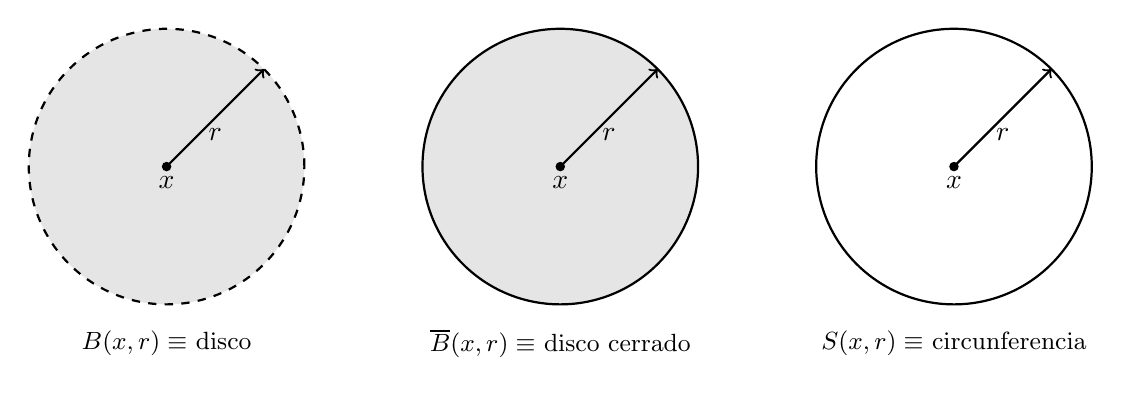
\begin{tikzpicture}
            \centering

            \def\radius{1.75}
            \def\incolor{gray!20}
            \def\angulo{45}

            % Desactiva los caracteres conflictivos
            \shorthandoff{>} % Para poner puntas de flecha

            \filldraw[dashed, fill=\incolor, thick] (-5,0) circle (\radius);
            \filldraw (-5,0) circle (1.5pt)  node[below] {$x$};
            \draw[thick, ->] (-5,0) -> ({-5+sin(\angulo)*\radius}, {cos(\angulo)*\radius}) node[midway, below] {$r$};
            \node at (-5,-2.25) {\small{$B(x,r) \equiv$ disco}};

            \filldraw[fill=\incolor, thick] (0,0) circle (\radius);
            \filldraw (0,0) circle (1.5pt)  node[below] {$x$};
            \draw[thick, ->] (0,0) -> ({sin(\angulo)*\radius}, {cos(\angulo)*\radius}) node[midway, below] {$r$};
            \node at (0,-2.25) {\small{$\overline{B}(x,r) \equiv$ disco cerrado}};

            \draw[thick] (5,0) circle (\radius);
            \filldraw (5,0) circle (1.5pt)  node[below] {$x$};
            \draw[thick, ->] (5,0) -> ({5+sin(\angulo)*\radius}, {cos(\angulo)*\radius}) node[midway, below] {$r$};
            \node at (5,-2.25) {\small{$S(x,r) \equiv$ circunferencia}};
        \end{tikzpicture}

        \item En $n=3$ tenemos:
        
        \vspace*{0.25cm}

        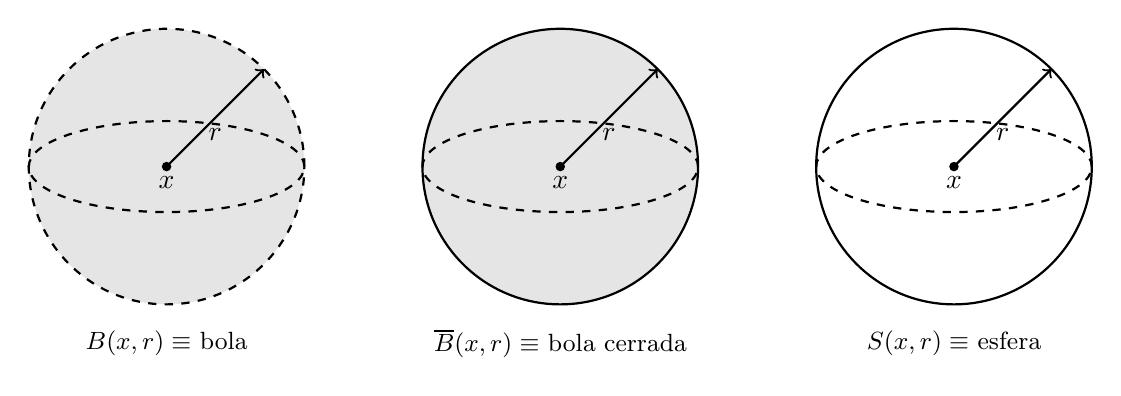
\begin{tikzpicture}
            \centering

            \def\radius{1.75}
            \def\incolor{gray!20}
            \def\angulo{45}

            % Desactiva los caracteres conflictivos
            \shorthandoff{>} % Para poner puntas de flecha

            \filldraw[dashed, fill=\incolor, thick] (-5,0) circle (\radius);
            \draw[dashed, thick] (-5,0) ellipse [x radius=\radius, y radius=0.33*\radius];
            \filldraw (-5,0) circle (1.5pt)  node[below] {$x$};
            \draw[thick, ->] (-5,0) -> ({-5+sin(\angulo)*\radius}, {cos(\angulo)*\radius}) node[midway, below] {$r$};
            \node at (-5,-2.25) {\small{$B(x,r) \equiv$ bola}};

            \filldraw[fill=\incolor, thick] (0,0) circle (\radius);
            \draw[dashed, thick] (0,0) ellipse [x radius=\radius, y radius=0.33*\radius];
            \filldraw (0,0) circle (1.5pt)  node[below] {$x$};
            \draw[thick, ->] (0,0) -> ({sin(\angulo)*\radius}, {cos(\angulo)*\radius}) node[midway, below] {$r$};
            \node at (0,-2.25) {\small{$\overline{B}(x,r) \equiv$ bola cerrada}};

            \draw[thick] (5,0) circle (\radius);
            \draw[dashed, thick] (5,0) ellipse [x radius=\radius, y radius=0.33*\radius];
            \filldraw (5,0) circle (1.5pt)  node[below] {$x$};
            \draw[thick, ->] (5,0) -> ({5+sin(\angulo)*\radius}, {cos(\angulo)*\radius}) node[midway, below] {$r$};
            \node at (5,-2.25) {\small{$S(x,r) \equiv$ esfera}};
        \end{tikzpicture}
    \end{itemize}
    \endsquare
\end{ejemplo}

\begin{ejemplo}
    En un conjunto $X \neq \emptyset$, se define la \textbf{distancia discreta} como 
    \begin{align*}
        d_{disc}(x,y) &=
        \left\{ 
        \begin{array}{ccc}
            0 & \text{si} & x=y\\
            1 & \text{si} & x\neq y
        \end{array}
        \right. 
    \end{align*}
    Con la distancia así definida tenemos:
    \begin{align*}
        B(x,y) &=
        \left\{ 
        \begin{array}{ccc}
            X & \text{si} & r>1\\
            \{x\} & \text{si} & r \leq 1
        \end{array}
        \right. \\\\
        \overline{B}(x,y) &=
        \left\{ 
        \begin{array}{ccc}
            X & \text{si} & r \geq 1\\
            \{x\} & \text{si} & r < 1
        \end{array}
        \right.\\\\
        S(x,y) &=
        \left\{ 
        \begin{array}{ccc}
            X \setminus \{x\} & \text{si} & r =1 \\
            \emptyset & \text{si} & r \neq 1\\
        \end{array}
        \right.
    \end{align*}
    \endsquare
\end{ejemplo}


\begin{ejemplo}\
    \begin{itemize}
        \item Si $d$ es una distancia en $X$ y $\lambda > 0$, entonces $\lambda \cdot d : X \times X \rightarrow [0,\infty)$ también es una distancia y $B_{\lambda d}(x,r) = B_d\left(x, \dfrac{r}{\lambda}\right)$.
        \item Sean $d$ y $\tilde{d}$ distancias en $X$ y $d \leq \tilde{d}$, entonces $B_d(x,r) \geq B_{\tilde{d}}(x,r)$.
    \end{itemize}
    \endsquare
\end{ejemplo}

\begin{definicion}
    $(X,d)$ e.m. Un subconjunto $U \subset X$ se dice \textbf{abierto métrico} si $U=\emptyset$ o si $\forall x \in U, \ \ \exists r > 0$ tal que $B(x,r) \subset U$.
    \endsquare
\end{definicion}

\begin{prop} %proposicion
    Si $(X,d)$ es un espacio métrico, entonces 
    \begin{gather*}
        \cc{T}_d=\{U \subset X : U \text{ es un abierto métrico en }(X,d)\} \subset \cc{P}(X)
    \end{gather*}
    es una topología en $X$ que llamamos la \textbf{topología métrica} en $(X,d)$.

    \begin{proof}\
        Veamos que $\cc{T}_d$ así definida verifica las propiedades de una topología:
        \begin{enumerate}[label=(A\arabic*)]
            \item $\emptyset$, $X\in \cc{T}_d$ trivialmente (ya que $X\subset X$).
            \item Sea $\{U_i\}_{i\in I}\subset \cc{T}_d$. Tendremos que ver si se verifica que $\bigcup\limits_{i\in I}U_i \in \cc{T}_d$. Para ello estudiemos los dos casos posibles:
            
            Si $\bigcup\limits_{i\in I}U_i = \emptyset \Rightarrow \bigcup\limits_{i\in I}U_i \in \cc{T}_d$.

            Si $\bigcup\limits_{i\in I}U_i \neq \emptyset$, entonces podemos considerar $x \in \bigcup\limits_{i\in I}U_i \Rightarrow \exists i \in I : x \in U_i \in \cc{T}_d \Rightarrow \exists r>0 : B(x,r) \subset U_i \subset \bigcup\limits_{i\in I}U_i \Rightarrow \bigcup\limits_{i\in I}U_i\in \cc{T}$.

            \item Sean $U_1, U_2 \in \cc{T}_d$. ¿Se verifica que $U_1 \cap U_2 \in \cc{T}_d$? De nuevo veamos los casos posibles:
            
            Si $U_1 \cap U_2 = \emptyset$, entonces se verifica trivialmente.

            Si $U_1 \cap U_2 \neq \emptyset$, entonces podemos considerar $x\in U_1 \cap U_2 \Rightarrow \exists r_1,r_2>0: B(x,r_1)\subset U_1$ y $B(x,r_2)\subset U_2 \Rightarrow B(x, \min\{r_1, r_2\}) \subset U_1 \cap U_2$, es decir existe una bola abierta en la intersección que contiene al punto luego $U_1 \cap U_2 \in \cc{T}_d$.
        \end{enumerate}
    \end{proof}
\end{prop}

\begin{definicion}
    Se llama \textbf{topología usual de $\bb{R}^n$}, $\cc{T}_u$, a la topología métrica en $\bb{R}^n$ con la distancia usual, es decir,
    $U \subset \bb{R}^n$ es abierto en $(\bb{R}^n, \cc{T}_u)$ si $U=\emptyset$ o si $\forall x \in U \ \ \exists r>0 : B(x,r) \subset U$.
    \endsquare
\end{definicion}

\begin{prop}
    $(X,d)$ e.m. Se cumplen:
    \begin{enumerate}
        \item[(i)] Las bolas abiertas en $(X,d)$ son abiertos.
        \item[(ii)] Todo abierto no vacío en $(X,d)$ se puede escribir como unión de bolas abiertas y como unión de bolas cerradas.
    \end{enumerate}


    \begin{proof}\
        \begin{enumerate}
            \item[(i)] Sea $x\in X$, $r>0$, ¿$B(x, r)\in \cc{T}_d$?
            
            Sea $y \in B(x,r) \Rightarrow d(x,y)<r \Rightarrow \exists \veps>0 : d(x,y) + \veps <r \Rightarrow B(y, \veps)\subset B(x,r)$. Para ver esta última implicación tenemos que si tomamos un $z \in B(y, \veps)\Rightarrow d(x,z) \leq d(x,y) + d(y,z) < d(x,y) + \veps < r \Rightarrow z \in B(x,r)$.

            \begin{center}
                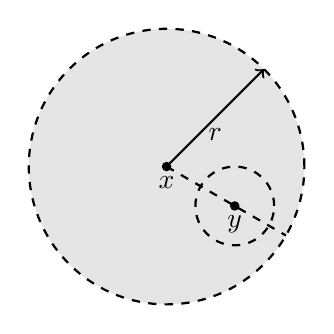
\begin{tikzpicture}
                    \centering
        
                    \def\radius{1.75}
                    \def\incolor{gray!20}
                    \def\angulo{45}
        
                    % Desactiva los caracteres conflictivos
                    \shorthandoff{>} % Para poner puntas de flecha
        
                    \filldraw[dashed, fill=\incolor, thick] (0,0) circle (\radius);
                    \filldraw (0,0) circle (1.5pt)  node[below] {$x$};
                    \draw[thick, ->] (0,0) -> ({sin(\angulo)*\radius}, {cos(\angulo)*\radius}) node[midway, below] {$r$};
                    \def\angulo{120}
                    \draw[thick, dashed] (0,0) -- ({sin(\angulo)*\radius}, {cos(\angulo)*\radius});

                    \filldraw ({sin(\angulo)*1}, {cos(\angulo)*1}) circle (1.5pt)  node[below] {$y$};

                    \def\radius{0.5}
                    \draw[dashed, thick] ({sin(\angulo)*1}, {cos(\angulo)*1}) circle (\radius);
        
                \end{tikzpicture}
            \end{center}
            
            \item[(ii)] Sea $U \in \cc{T}_d \Rightarrow \forall x \in U \ \ \exists r_x >0$ tal que $B(x,r_x)\subset U \Rightarrow U = \bigcup\limits_{x\in U}B(x, r_x) = \bigcup\limits_{x\in U}\overline{B}\left(x, \frac{r_x}{2}\right)$.
            
        \end{enumerate}
    \end{proof}
\end{prop}

\begin{coro}
    En $(X,d)$ tenemos 
    \begin{gather*}
        \cc{T}_d=\{\emptyset\}\cup\{U \subset X : U \text{ es unión de bolas abiertas}\}
    \end{gather*}
    \endsquare
\end{coro}

\begin{ejemplo}\
    \begin{itemize}
        \item $(X,d)$ e.m. En general, no todo abierto es una bola. Pir ejemplo la unión de bolas no concéntricas.
        \item No todo conjunto en $(\bb{R}^n, \cc{T}_u)$ es abierto. Por ejemplo $\{x\}\subset \bb{R}^n$ no es abierto.
        \item En $(\bb{R}, \cc{T}_u)$ los únicos intervalos abiertos (topológicamente) son los intervalos abiertos, es decir, los del tipo $\bb{R}=(-\infty, +\infty)$, $(a,b)$ con $a<b$, $(-\infty, a)$ y $(b, +\infty)$.
        \item En $(X, d)$, en general la intersección infinita de abiertos no es abierto. Por ejemplo, $\bigcap\limits_{n\in \bb{N}}\left(\frac{-1}{n}, \frac{1}{n}\right) = \{0\}$ que no es abierto.
        \item $X\neq \emptyset$, $\cc{T}_{d_{disc}}=\cc{T}_{disc}$ (la topología asociada a la distancia discreta es la distancia discreta).
    \end{itemize}
    \endsquare
\end{ejemplo}

\begin{definicion}
    Sean $X\neq \emptyset$ y $d_1, d_2$ distancias en $X$. Decimos que $d_1$ y $d_2$ son \textbf{equivalentes} si existen $a,b>0$ tal que 
    \begin{gather*}
        a \cdot d_1(x,y) \leq d_2(x,y) \leq b \cdot d_1(x,y) \ \ \ \forall x,y \in X
    \end{gather*}
    \endsquare
\end{definicion}

\begin{prop}
    Si $d_1, d_2$ son distancias en $X \neq \emptyset$ y existe $a>0$ tal que $a \cdot d_1(x,y) \leq d_2(x,y) \ \ \ \forall x,y \in X$, entonces $\cc{T}_{d_1} \subset \cc{T}_{d_2}$. En particular, si $d_1$ y $d_2$ son equivalentes, entonces $\cc{T}_{d_1} = \cc{T}_{d_2}$.


    \begin{proof}
        Sea $U\in \cc{T}_{d_1}$, $U \neq \emptyset$, ¿$U\in \cc{T}_{d_2}$?

        Sea $x \in U \in \cc{T}_{d_1} \Rightarrow \exists r>0: B_{d_1}(x,r)\subset U$. Como $a \cdot d_1 \leq d_2 \Rightarrow B_{d_2}(x,a\cdot r)\subset B_{d_1}(x,r)$. Para verlo, tomamos $y\in B_{d_2}(x,a\cdot r) \Rightarrow d_2(x,y)<a\cdot r \Rightarrow a \cdot d_1(x,y)<r \Rightarrow y \in B_{d_1}(x,r)$. Por tanto, $B_{d_1}(x,r)\subset U \Rightarrow U \in \cc{T}_{d_2}\Rightarrow T_{d_1}\subset \cc{T}_{d_2}$.\\
    \end{proof}
\end{prop}

\begin{definicion}
    Un e.t. $(X,\cc{T})$ se dice \textbf{metrizable} si existe una distancia $d$ en $X$ tal que $\cc{T}= \cc{T}_d$.
    \endsquare
\end{definicion}

\begin{ejemplo}\ 
    \begin{itemize}
        \item $(\bb{R}^n, \cc{T}_u)$ es metrizable.
        \item $(X, \cc{T}_{disc})$ es metrizable.
    \end{itemize}
    \endsquare
\end{ejemplo}

\begin{ejercicio}
    Si $(X,\cc{T})$ es un e.t. metrizable, entonces cumple la condición de Hausdorff:
    \begin{gather*}
        \forall x,y\in X, x\neq y, \ \ \exists U,V \in \cc{T} \text{ tal que }x\in U,\ y\in V \text{ y } U \cap V = \emptyset
    \end{gather*}

    Por ser metrizable, sabemos que $\cc{T}=\cc{T}_d$ donde $d:X \to [0,\infty)$ es una distancia. Por tanto, para cada $x,y\in X$ con $x\neq y$ tengo $d(x,y)>0$. Puedo considerar entonces $r=\dfrac{d(x,y)}{2}$. Tengo entonces $U=B(x,r)$ y $V=B(y,r)$. Es claro que $x\in U$ y $y\in V$. Veamos que $U$ y $V$ son disjuntos. Tengo $U\cap V =\{z\in X : d(z,x)<r ,d(z,y)<r\}$. Supongamos que este conjunto no es vacío, en cuyo caso tendría que $\exists z \in X$ tal que $d(z,x)<r$ y $d(z,y)<r$. Por tanto, $d(z,x)+d(z,y)<2r = d(x,y)$ lo cual incumple la desigualdad triangular. Llegamos a contradicción y por tanto $U\cap V=\emptyset$.
    \endsquare
\end{ejercicio}

\begin{ejemplo}\
    \begin{itemize}
        \item $(X,\cc{T}_t)$ no es metrizable si $\#X>2$ (cardinal del conjunto) ya que no verifica la condición de Hausdorff.
        \item $(X, \cc{T}_{x_0})$ no es metrizable por la misma razón (ya que la intersección de cualesquiera dos abiertos va a contener a $x_0$).
        \item $(X, \cc{T}_{CF})$ no es metrizable si $X$ es infinito (aplicar las leyes de morgan para la intersección).
        \item $(X, \cc{T}_{CN})$ no es metrizable si $X$ no es numerable.
        \item $(\bb{R}, \{\emptyset, \bb{R}, \bb{Q}, \bb{R}\setminus \bb{Q}\})$.
        \item La topología de Sierpinski tampoco es metrizable (ya que el único abierto que contiene a $b$ es el total).
        \item La topología de Sorgenfrey $(\bb{R}, \cc{T}_S)$ cumple la propiedad de Hausdorff.
    \end{itemize}
    \endsquare
\end{ejemplo}

\section{Comparación de Topologías}
\begin{definicion}
    Sean $X\neq \emptyset$ un conjunto y $\cc{T}_1$, $\cc{T}_2$ dos topologías en $X$. Diremos que $\cc{T}_2$ es \textbf{más fina} que $\cc{T}_1$ o que $\cc{T}_1$ es \textbf{menos fina} que $\cc{T}_2$ si $\cc{T}_1\subseteq \cc{T}_2$ y lo notamos como $\cc{T}_1 \leq \cc{T}_2$.
    \endsquare
\end{definicion}

\begin{ejemplo}\
    \begin{itemize}
        \item $X \neq \emptyset$,\ $\cc{T}_{CF}\leq \cc{T}_{CN}$.
        \item $(X,\cc{T})$ e.t, entonces $\cc{T}_t \leq \cc{T} \leq \cc{T}_{disc}$ 
        % (ya que todas las topologías contienen a la trivial)
        \item Si $\cc{T}_1 \leq \cc{T}_2$ y $\cc{T}_2\leq \cc{T}_1$, entonces $\cc{T}_1= \cc{T}_2$ (por doble inclusión).
        \item En general si tenemos dos topologías en $X$, no siempre son comparables. Por ejemplo la topología del punto incluida en dos puntos distintos: 
        \begin{gather*}
            0,1\in \bb{R}\ \ \ (\bb{R}, \cc{T}_0), (\bb{R},\cc{T}_1)
        \end{gather*}
        Veamos que $\cc{T}_0 \nleq \cc{T}_1$, ya que $\{0\}\notin \cc{T}_1$, y por el mismo motivo (pero con el 1) tenemos $\cc{T}_1\nleq \cc{T}_0$.

        Otro ejemplo sería $(\bb{R}, \cc{T}_u)$, $(\bb{R},\cc{T}_{x_0})$ ya que $\{x_0\}\in \cc{T}_{x_0}$, $\{x_0\}\notin \cc{T}_u\Rightarrow \cc{T}_{x_0\nleq \cc{T}_u}$
        Igualmente $(x_0+1,x_0+2)\in \cc{T}_u$ y $(x_0+1,x_0+2)\in \cc{T}_{x_0} \Rightarrow \cc{T}_u \nleq topoº_{x_0}$
        \item En $\bb{R}$, $\cc{T}_u\leq \cc{T}_{Sorgenfrey}$.
        \item $(X,d)$, $(X,d')$, $d \leq d' \Rightarrow \cc{T}_d \leq \cc{T}_{d'}$.
    \end{itemize}
    \endsquare
\end{ejemplo}

\section{Cerrados}

\begin{definicion}
    Sea $(X,\cc{T})$ un e.t. Diremos que un conjunto $F\subset X$ es \textbf{cerrado} en $(X,\cc{T})$ si $X\subset F \in \cc{T}$. Denotamos por $\cc{C}_{\cc{T}}$ a la familia de todos los cerrados en $(X,\cc{T})$.
    \endsquare
\end{definicion}

\begin{propiedades}\ 
    \begin{enumerate}
        \item[\objetivo{C1}] $\emptyset, X \in \cc{C}_{\cc{T}}$.
        \item[\objetivo{C2}] Si $\{F_i\}_{i\in I}\subset \cc{C}_{\cc{T}}$, entonces $\bigcap\limits_{i\in I}F_i \in \cc{C}_{\cc{T}}$.
        \item[\objetivo{C3}] Si $F_1, F_2" \in \cc{C}_{\cc{T}}$, entonces $F_1 \cup F_2 \in \cc{C}_{\cc{T}}$
    \end{enumerate}
    Por inducción, de \apuntar{C3} tenemos que la unión finita de cerrados es cerrada.\\
\end{propiedades}

\begin{observacion}\
    \begin{itemize}
        \item $U\in \cc{T}\sii X \setminus U \in \cc{C}_{\cc{T}}$, $F\in \cc{C}_{\cc{T}} \sii X\setminus F \in \cc{T}$.
        \item $\cc{T}_1 \leq \cc{T}_2\sii \cc{C}_{\cc{T}_1}\subseteq \cc{C}_{\cc{T}_2}$. Esto además implica que $\cc{T}_1=\cc{T}_2 \sii \cc{C}_{\cc{T}_1} = \cc{C}_{\cc{T}_2}$. Esto nos dice que para conocer una topología basta con conocer la familia de sus cerrados.
        \item En general, puede haber conjntos que no sean ni abiertos ni cerrados. Por ejemplo, en $(\bb{R}, \cc{T}_u)$, tenemos que $[0,1)\notin \cc{T}_u\cup \cc{C}_{\cc{T}_u}$.
        \item En $(X, \cc{T}_{x_0})$ tenemos que $\cc{T}_{x_0}\cup \cc{C}_{\cc{T}_{x_0}} = \cc{P}(X)$ y además $\cc{T}_{x_0}\cap \cc{C}_{\cc{T}_{x_0}}=\{\emptyset, X\}$.
        \item En general, la unión arbitraria de cerrados no es cerrado. Por ejemplo, $(\bb{R}, \cc{T}_u)$, tomamos $\bigcup\limits_{n\in \bb{N}}\left[-\frac{1}{n}, 3-\frac{1}{n}\right] = (0,3)$. Otro ejemplo sería $(\bb{R}, \cc{T}_{CF})$ considerando $\bigcup\limits_{n\in \bb{N}}\{n\}=\bb{N}$ que no es cerrado.
    \end{itemize}
    \endsquare
\end{observacion}
\begin{ejemplo}\
    \begin{itemize}
        \item Topología trivial: $\cc{T}_t=\{\emptyset, X\} \Rightarrow \cc{C}_{\cc{T}_t} = \cc{C}_t = \{\emptyset, X\}$.
        \item Topología discreta: $\cc{T}_{disc} = \cc{P}(X) \Rightarrow \cc{C}_{\cc{T}_{disc}} = \cc{C}_{disc} = \cc{P}(X)$.
        \item Topología del punto incluido: $x_o \in X$, $\cc{T}_{x_0}=\{\emptyset\} \cup \{U\subset X : x_0 \in U\} \Rightarrow \cc{C}_{\cc{T}_{x_0}} = \cc{C}_{x_0} = \{X\}\cup \{F \subset X : x_0 \notin F\}$
        \item Topología cofinita: $\cc{T}_{CF} = \{\emptyset\}\cup \{U\subset X : X \setminus U \text{ finito }\} \Rightarrow \cc{C}_{\cc{T}_{CF}}=\cc{C}_{CF}=\{X\}\cup \{F\subset X : F \text{ finito}\}$
        \item En ocasiones no es fácil describir $\cc{C}_{\cc{T}}$. Por ejemplo en $\cc{T}_u$ o $\cc{T}_{Sorgenfrey}$.
    \end{itemize}
    \endsquare
\end{ejemplo}

\begin{ejemplo} En un espacio métrico $(X, \cc{T}_d)$, las bolas cerradas y las esferas son cerrados.
    \begin{proof}\
        \begin{itemize}
            \item Sea $x\in X$, $r>0$, ¿$\overline{B}(x,r)\in \cc{C}_d$? Esto es equivalente a preguntarse ¿$X\setminus \overline{B}(x,r) \in \cc{T}_d$?
            
            Sea $y \in X\setminus\overline{B}(x,r) \Rightarrow d(x,y>r)$. Entonces $\exists \veps >0 : r+\veps < d(x,y)\Rightarrow B(y,\veps)\cap \overline{B}(x,r)=\emptyset \Rightarrow B(y,\veps)\subset X\setminus \overline{B}(x,r)\in \cc{T}_d \Rightarrow X\setminus \overline{B}(x,r)\in \cc{C}_{\cc{T}}$

            \item Sea $x\in X$, $r>0, $¿$S(x,r)\in \cc{C}_d$? Dado que $X\setminus S(x,r)=B(x,r)\cup (X\setminus \overline{B}(x,r))\in \cc{T}_d$ (por ser unión de abiertos).
        \end{itemize}
    \end{proof}
\end{ejemplo}

\begin{ejercicio}
    En $(\bb{R},\cc{T}_u)$ los únicos intervalos cerrados son los de la forma $(-\infty, a]$, $[b, +\infty)$, $\bb{R}=(-\infty, +\infty)$ y $[a,b]$ con $a<b$.\\

    Sabemos que los únicos abiertos en $\cc{T}_u$ son los intervalos de la forma $\bb{R}=(-\infty, +\infty)$, $(a,b)$ con $a<b$, $(-\infty, a)$ y $(b, +\infty)$.

    Es claro que $\bb{R}\in \cc{C}_{\cc{T}_u}$. 
    
    Tenemos que $\bb{R}\setminus(-\infty,a] = (a,+\infty)\in \cc{T}_u$, luego $(-\infty,a]\in \cc{C}_{\cc{T}_u}$. 
    
    De la misma forma, $\bb{R}\setminus[b,+\infty) = (-\infty,b)\in \cc{T}_u$, luego $[b,+\infty)\in \cc{C}_{\cc{T}_u}$

    Finalmente $\bb{R}\setminus [a,b]=(-\infty,a)\cup(b,+\infty)\in \cc{T}_u$ por ser unión de abiertos luego $[a,b]\in \cc{C}_{\cc{T}_u}$.

    Dado que ya han aparecido todos los tipos posibles de intervalos en $\bb{R}$, no habrá más intervalos cerrados que los ya mencionados (ya que cualquier otro tipo de intervalo es abierto).

    \endsquare
\end{ejercicio}

\begin{teo}
    Sea $X\neq \emptyset$ y $\cc{C}\subset \cc{P}(X)$ cumpliendo
    \begin{enumerate}
        \item[\apuntar{C1}] $\emptyset, X \in \cc{C}$.
        \item[\apuntar{C2}] Si $\{F_i\}_{i\in I}\subset \cc{C}$, entonces $\bigcap\limits_{i\in I}F_i \in \cc{C}$.
        \item[\apuntar{C3}] Si $F_1, F_2" \in \cc{C}$, entonces $F_1 \cup F_2 \in \cc{C}$
    \end{enumerate}

    Entonces existe una única topología $\cc{T}$ en $X$ tal que $\cc{C}_{\cc{T}}=\cc{C}$.

    \begin{proof}
        La existencia queda probada definiendo $\cc{T}=\{U\subset X : X \setminus U \in \cc{C}\}$.
        La unicidad es inmediata ya que si $\cc{C}_{\cc{T'}}=\cc{C}_{\cc{T}}\Rightarrow \cc{T}=\cc{T}'$.\\
    \end{proof}
\end{teo}

\section{Bases de topología}

\begin{definicion}
    Sea $(X,\cc{T})$ un e.t. Una familia de abiertos $\cc{B}\subset \cc{T}$ es una \textbf{base} de la topología $\cc{T}$ si $\forall U \in \cc{T}$\ \ \ $\exists \{B_i\}\subset \cc{B}$ tal que $U=\bigcup\limits_{i\in I}B_i$.

    A los elementos de $\cc{B}$ se les llama \textbf{abiertos básicos}.
    \endsquare
\end{definicion}

\begin{observacion}\
    \begin{itemize}
        \item Ni $\cc{B}$ ni la familia $\{B_i\}_{i\in I}$ tienen que ser finitas o numerables
        \item La forma de escribir $U=\bigcup\limits_{i\in I} B_i$ puede no ser única.
        \item $\cc{T}$ es base de $\cc{T}$ (trivialmente).
        \item Si $\cc{B}\subset \cc{B}'\subset \cc{T}$ con $\cc{B}$, entonces $\cc{B}'$ es base de $\cc{T}$.
    \end{itemize}
    \endsquare
\end{observacion}

\begin{prop}
    Sea $(X,\cc{T})$ un e.t y $\cc{B}\subset \cc{T}$ una familia de abiertos. Son equivalentes:
    \begin{enumerate}
        \item[(i)] $\cc{B}$ es base de $\cc{T}$.
        \item[(ii)] $\forall U \in \cc{T}$,\ \ $U \neq \emptyset$\ \ $\forall x\in U$\ \ $\exists B \in \cc{B}$ tal que $x\in B \subset U$ (si tenemos un abierto de la topología podemos encontrar para cada punto suyo un abierto básico contenido en el abierto y que contiene al punto).
    \end{enumerate}

    \begin{proof}\
        \begin{itemize}
            \item[(i)$\Rightarrow$(ii)] Sea $U\in \cc{T}$, $U\neq \emptyset$. Sea $x \in U \Rightarrow  U = \bigcup\limits_{i\in I}B_i$ con $B_i \in \cc{B}\Rightarrow \exists i\in I$ tal que $x\in B_i=B_x\subset U$
            \item[(ii)$\Rightarrow$(i)] Sea $U\in \cc{T}$.
            \begin{itemize}[label=-]
                \item Si $U=\emptyset\Rightarrow U=\bigcup\limits_{i\in \emptyset}B_i=\emptyset$
                \item Si $U \neq \emptyset \Rightarrow \forall x \in U$\ \ $\exists B_x\in \cc{B}$ tal que $x\in B_x \subset U\Rightarrow U = \bigcup\limits_{x\in U}B_x$
            \end{itemize}
        \end{itemize} 
    \end{proof}
\end{prop}


\begin{ejemplo}\
    \begin{itemize}
        \item Sea $(X,\cc{T}_d)$ un e.m. La familia $base=\{B(x,r):x\in X, r>0\}$ de todas las bolas abiertas es una base de $\cc{T}_d$.
        \item En $(\bb{R},\cc{T}_u)$, $\cc{B}_u=\{(a,b):a<b\}$ es base de $\cc{T}_u$ y se le llama \textbf{base usual}.
        \item En $(\bb{R},T_u)$, $\cc{B}=\{(a,b): a,b\in \bb{Q},\ a<b\}$ es base de $\cc{T}_u$ (por la densidad de $\bb{Q}$ en $\bb{R}$).
        \item En $(\bb{R}^n, \cc{T}_u)$, $\cc{B}_u=\{B(x,r): x\in \bb{R}^n, r>0\}$ es la base usual. $(\bb{R}^n, \cc{T}_u)$, $\cc{B}_u=\{B(x,r): x\in \bb{R}^n, r\in \bb{Q}, r>0\}$ también es base de $\cc{T}_u$ (numerable).
        \item En $(X,\cc{T}_t)$, $\cc{B}=\{X\}$ es base (la única que no contiene al vacío).
        \item $(X,\cc{T}_d)$, $\cc{B}=\{\{x\}: x\in X\}\subset \cc{T}$ es base de $\cc{T}_{disc}$. Es la más económica ya que si $\cc{B}'$ es base, entonces $\cc{B}\subset \cc{B}'$.
        \begin{proof}
            Sea $\{x\}\in \cc{T}_{disc}$, como $\cc{B}'$ es base podemos considerar $x\in \{x\}$ y entonces $\exists B \in \cc{B}'$ tal que $x\in B \subset \{x\}$ y entonces $B=\{x\}\subset \cc{B}'$ $\forall x \in X\Rightarrow \cc{B}\subset \cc{B}'$
        \end{proof}
        \item $(X, \cc{T}_{x_0})$, $x_0 \in X \neq \emptyset$, $\cc{B}=\{\{x,x_0\}: x\in X\}$ es una base. Esta es la base más económica.
        \item $(\bb{R}, \cc{T}_{Sorgenfrey})$ (recordemos que $U \in \cc{T}_S \sii \forall x \in U,\ \ \exists \veps : [x, x+\veps)\subset U$). $\cc{B}=\{[x,x+\veps): x\in \bb{R}, \veps>0\}$ es base. $\cc{B}'=\{[x,x+\veps): x\in \bb{Q}, \veps\in \bb{Q}, \veps>0\}$ no lo es (ya que tomando un intervalo de la forma $[x,x+\veps)$ con $x\in \bb{Q}$ entonces no existe ningún elemento de $\cc{B}'$ que contenga a $x$ y quede enmedio).
    \end{itemize}
    \endsquare
\end{ejemplo}

\begin{teo}
    Sea $(X,\cc{T})$ un espacio topológico y $\cc{B}$ una base suya. Entonces:
    \begin{enumerate}
        \item[\objetivo{B1}] $X=\bigcup\limits_{B\in \cc{B}}B$
        \item[\objetivo{B2}] Si $B_1,B_2\in \cc{B}$,\ $x\in B_1\cap B_2$, entonces $\exists B_3 \in \cc{B}$ con $x\in B_3 \subset B_1 \cap B_2$
    \end{enumerate}

    \begin{proof}\
        \begin{enumerate}
            \item[\apuntar{B1}] Trivial
            \item[\apuntar{B2}] Tenemos $x\in B_1\cap B_2\in \cc{T}$ entonces, como $\cc{B}$ es base $\exists B_3=B_x \in \cc{B}$ con $x\in B_3 \subset B_1 \cap B_2$.
        \end{enumerate}
    \end{proof}
\end{teo}

\begin{teo}
    Sean $X\neq \emptyset$ un conjunto y $\cc{B}\subset \cc{P}(X)$ cumpliendo:
    \begin{enumerate}
        \item[\apuntar{B1}] $X=\bigcup\limits_{B\in \cc{B}}B$
        \item[\apuntar{B2}] Si $B_1,B_2\in \cc{B}$,\ $x\in B_1\cap B_2$, entonces $\exists B_3 \in \cc{B}$ con $x\in B_3 \subset B_1 \cap B_2$
    \end{enumerate}
    Entonces existe una única topología $\cc{T}(\cc{B})$ en $X$ tal que $\cc{B}$ es base de $\cc{T}(\cc{B})$. Además,
    \begin{align*}
        \cc{T}(\cc{B})&=\{\emptyset\}\cup\{U\subset X : \exists \{B_i\}_{i\in I}\subset \cc{B} \text{ con } U = \bigcup\limits_{i\in I}B_i\}\\
        &=\{\emptyset\}\cup \{U\in X:\forall x\in U\ \ \exists B=B_x\in \cc{B} \text{ con } x\in B\subset U \}
    \end{align*}
    Además, $\cc{T}(\cc{B})$ es la topología menos fina conteniendo a $\cc{B}$, es decir, si $(X,\cc{T}')$ es un e.t y $\cc{B}\subset \cc{T}'$, entonces $\cc{T}(\cc{B})\leq \cc{T}'$. A esta topología se le llama la \textbf{topología generada} por $\cc{B}$.

    \begin{proof}
        Empezaremos por probar la existencia. Para ello tendremos que ver que $\cc{T}(\cc{B})$ es una topología, probando que verifica las propiedades de las topologías:
        \begin{enumerate}[label=(A\arabic*)]
            \item $\emptyset\in \cc{T}(\cc{B})$ por la definición de $\cc{T}(\cc{B})$. Por \apuntar{B1}, tenemos también que $X\in \cc{T}(\cc{B})$.
            \item Sea $\{U_i\}_{i\in I}\subset \cc{T}(\cc{B})$ y sea $x\in \bigcup\limits_{i\in I}U_i\Rightarrow \exists i \in I : x\in U_i\in \cc{T}(\cc{B})$ por lo que $\exists B_x\in \cc{B}$ tal que $x \in B_x \subset U_i\subset \bigcup_{i\in I}U_i\Rightarrow \bigcup\limits_{i\in I}U_i \in \cc{T}(\cc{B})$.
            \item Sean $U_1, U_2 \in \cc{T}(\cc{B})$ (si la intersección es vacía es trivial). Consideramos $x\in U_1\cap U_2\Rightarrow \exists B_1, B_2 \in \cc{B}$ con $x \in B_1 \subset U$ y $x_\in B_2\subset U_2$ por tanto $x\in B_1 \cap B_2 \subset U_1 \cap U_2$. Por \apuntar{B2}, existe un $B_2\in \cc{B}$ tal que $x\in B_3 \subset B_1\cap B_2 \subset U_1 \cap U_2$ por lo que $U_1\cap U_2\in \cc{T}(\cc{B})$.
        \end{enumerate}
        Con esto queda probado que es una topología. Tendremos que ver ahora que $\cc{B}$ es base de $\cc{T}(\cc{B})$. Para ello empiezo viendo que $\cc{B}\subset \cc{T}$. Por la segunda defición de $\cc{T}(\cc{B})$, esto es evidente. Como verifica las hipótesis del Teorema 1.7, es base de $\cc{T}(\cc{B})$.\\

        Veamos ahora la unicidad. Sea $(X, \cc{T}')$ un e.t. con $\cc{B}$ base de $\cc{T}'$. Tendré que ver que $\cc{T}'=\cc{T}$. Sea $\emptyset\neq U\subset X \Rightarrow U\in \cc{T}'\sii \forall x \in U\ \ \exists B\in \cc{B}$ con $x\in \cc{B}\subset U \sii U\in \cc{T}(\cc{B})$ ya que $\cc{B}$ es base de $\cc{T}'$.\\

        Nos queda ver que es la menos fina conteniendo a $\cc{B}$. Para ello, sea $(X,\cc{T}')$ un e.t. tal que $\cc{B}\subset \cc{T}'$, entonces por \apuntar{A2} tenemos que $\cc{T}(\cc{B})\subset \cc{T}'$, lo cual es equivalente a decir que $\cc{T}(\cc{B})\leq \cc{T}'$.\\
    \end{proof}
\end{teo}

\begin{ejemplo}\
    \begin{itemize}
        \item Si $X=\{a,b\}$ y $\cc{B}=\{\{a\}\}$ no es base de ninguna topología en $X$ (ya que no cumple \apuntar{B1}).
        \item Si $X=\{a,b,c\}$ y $\cc{B}=\{\{a,b\},\{b,c\}\}$. Esta base verifica \apuntar{B1} pero no \apuntar{B2} (tomando $x=b$ se ve facilmente). %TODO 
        \item Si $X=\bb{R}$ y $\cc{B}=\{[a,b]:a<b\}$. Si tomamos dos intervalos $[0,1]\cap [1,2]$, su intersección es $\{1\}$ y por tanto no verifica \apuntar{B2} (tomando $x=1$).
        \item Si $X=\bb{R}$ y $\cc{B}=\{[a,b]:a\leq b\}$ es base de una topología, $\cc{T}(\cc{B})$ en $\bb{R}$. Además, $\cc{T}(\cc{B})=\cc{T}_{disc}$.
    \end{itemize}
    \endsquare
\end{ejemplo}

\begin{prop}
    Sean $X\neq \emptyset$ y $\cc{T}_1, \cc{T}_2$ topologías en $X$ con bases $\cc{B}_1$ y $\cc{B}_2$ respectivamente. Equivalen:
    \begin{enumerate}
        \item[(i)] $\cc{T}_1\leq \cc{T}_2$.
        \item[(ii)] $\forall B_1 \in \cc{B}_1,\ \ x \in B_1,\ \ \exists B_2 \in \cc{B}_2$ con $x\in B_2 \subset B_1$.
    \end{enumerate}
    \begin{proof}\
        \begin{enumerate}
            \item[(i)$\Rightarrow$(ii)] Sea $B \in \cc{B}_1$. Por (i), $\cc{B}_1 \subset \cc{T}_1 \subset \cc{T}_2$ y como $\cc{B}_2$ es base de $\cc{T}_2$, aplicando la definición de base tengo que $\exists B_2 \in \cc{B}_2$ con $x\in B_2 \subset B_1$.
            \item[(ii)$\Rightarrow (i)$] Por (ii) tenemos que $\cc{B}_1\subset \cc{T}_2\Rightarrow \cc{T}(\cc{B}_1)\leq \cc{T}_2$ (por el Teorema 1.7) %TODO
             y entonces $\cc{T}_1=\cc{T}(\cc{B}_1)\leq \cc{T}_2$.
        \end{enumerate}
    \end{proof}
\end{prop}

\begin{ejemplo}\
    \begin{itemize}
        \item En $\bb{R}$, $\cc{T}_u \leq \cc{T}_{Sorgenfrey}$.
        \item Ejercicios 1 y 2 de la relación.
    \end{itemize}
    \endsquare
\end{ejemplo}

\begin{prop}
    Sean $X\neq \emptyset$ y $S\subset \cc{P}(X)$, $S\neq \emptyset$, Entonces, 
    \begin{gather*}
        \cc{B}(S)=\left\{\bigcap\limits_{i\in I}: I \text{ finito, }S_i \in S\ \ \forall i \in I\right\}
    \end{gather*}
    Es base de una única topología $\cc{T}(S)=\cc{T}(\cc{B}(S))$ en $X$. A esta topología la llamaremos la \textbf{topología generada} por $S$ y es la topología menos fina que contiene a $S$, es decir, si $(X,\cc{T}')$ es un e.t. y $S\subset \cc{T}'$, entonces $\cc{T}(S)\leq \cc{T}'$.\\

    Decimos que $S$ es una \textbf{subbase} de $\cc{T}(S)$.

    \begin{proof}
        Tendremos que comprobar \apuntar{B1} y \apuntar{B2} y que es la menos fina.
    \end{proof}
\end{prop}

\begin{ejemplo}\
    \begin{itemize}
        \item Toda base $(X,\cc{T})$ es subbase de $(X,\cc{T})$.
        \item $S=\{X\}$ es subbase de $\cc{T}_t$.
        \item En $\bb{R}$, $S=\{(a,+\infty):a\in \bb{R}\}\cup \{(-\infty,b): b\in \bb{R}\}$ es subbase de $\cc{T}_u$.
    \end{itemize}
    \endsquare
\end{ejemplo}

\section{Entornos}

\begin{definicion}
    Sea $(X, \cc{T})$ un e.t y $x\in X$. Diremos que un conjunto $N\subset X$ es un \textbf{entorno} de $x$ si $\exists U \in \cc{T}$ con $x\in U \subset N$.\\

    Denotamos $\cc{N}_x = \{N\subset X : N \text{ es entorno de }x\}$ y lo llamamos \textbf{sistema de entornos} del punto $x$ en $(X,\cc{T})$.
    \endsquare 
\end{definicion}

\begin{ejemplo}\
    \begin{itemize}
        \item En $(\bb{R}, \cc{T}_u)$, $[0,1)\in \cc{N}_x$ para todo $x\in (0,1)$, pero no es entorno de $0$ ni de $1$.
    \end{itemize}
    \endsquare
\end{ejemplo}

\begin{observacion}\
    \begin{itemize}
        \item $X\in \cc{N}_x$\ \ $\forall x \in X\Rightarrow \cc{N}_x\neq \emptyset$\ \ $\forall x\in X$.
        \item Si $x\in U \in \cc{T}\Rightarrow U\in \cc{N}_x$
        \item Puede ocurrir que exista $N\subset \cc{N}_x$ con $N\notin \cc{T}$.
    \end{itemize}
    \endsquare
\end{observacion}

\begin{prop}
    Sea $(X,\cc{T})$ un e.t., $U\subset X$. Equivalen:
    \begin{enumerate}
        \item[(i)] $U\in \cc{T}$.
        \item[(ii)] $U\in \cc{N}_x$\ \ $\forall x \in U$.
    \end{enumerate}

    \begin{proof}\
        \begin{enumerate}
            \item[(i)$\Rightarrow$ (ii)] Si $U\in \cc{T}$, entonces $U\in \cc{N}_x$\ \ $\forall x\in U$
            \item[(ii)$\Rightarrow$ (i)] $\forall x \in U $\ \ $\exists U_x \in \cc{T}$ con $x\in U_x\subset U \Rightarrow U = \bigcup\limits_{x\in U}U_x \in \cc{T}$.
        \end{enumerate}
    \end{proof}
\end{prop}

\begin{ejemplo}\
    \begin{itemize}   
        \item $(X,\cc{T}_t)$, $\cc{N}_x=\{X\}$\ \ $\forall x \in X$.
        \item $(X,\cc{T}_{disc})$, $\cc{N}_x=\{N\subset X : x\in N\}$
        \item $(X,\cc{T}_{x_0})$, $\cc{N}_x = \{N \subset X : x_0,x\in N\}$
        \item $(X,d)$, $\cc{N}_x = \{N\subset X : \exists \veps > 0 \text{ con } B(x,r)\subset N\}$. En particular, $\overline{B}(x,r)\in \cc{N}_x$.
    \end{itemize}
    \endsquare
\end{ejemplo}

\begin{prop}
    Sea $(X,\cc{T})$ e.t., $x\in X$. Entonces:
    \begin{enumerate}
        \item[\objetivo{N1}] $\cc{N}_x \neq \emptyset$\ \ $\forall x \in X$.
        \item[\objetivo{N2}] Si $N \in \cc{N}_x$, entonces $x\in N$.
        \item[\objetivo{N3}] Si $N \in \cc{N}_x$ y $N\subset N'$, entonces $N'\in \cc{N}_x$.
        \item[\objetivo{N4}] Si $N,N'\in \cc{N}_x$, entonces $N\cap N' \in \cc{N}_x$.
        \item[\objetivo{N5}] Si $N\in \cc{N}_x$, entonces $\exists N'\in \cc{N}_x$ con $N'\subset N$ y $N\in \cc{N}_y$\ \ $\forall y \in N'$.  
    \end{enumerate}
    \begin{proof}\
        \begin{enumerate}
            \item[\apuntar{N5}] $N\in \cc{N}_x\Rightarrow \exists U \in \cc{T}$ con $x\in U\subset N$. Tomamos $U=N'$ y se verifica que $x\in U \in \cc{N}_x$. Además $U\subset N$ y tendré que ver que $N\in \cc{N}_y$\ \ $\forall y \in U$. Como $U\in \cc{T}\Rightarrow U\in \cc{N}_y$\ \ $\forall y \in U \overset{\apuntar{N3}}{\Rightarrow} N\in \cc{N}_y$\ \ $\forall y \in U$.
        \end{enumerate}
    \end{proof}
\end{prop}

\begin{prop}
    (Hausdorff, 1914) Sean $X\neq \emptyset$ un conjunto y supongamos que tenemos $\forall x \in X$ una familida $\cc{M}_x\subset \cc{P}(X)$ cumpliendo \apuntar{N1},\dots,\apuntar{N5}. Entonces existe una única topología $\cc{T}$ en $X$ cuyos sustemas de entornos $\cc{N}_x$ coinciden con $\cc{M}_x$\ \ $\forall x \in X$ (es decir, $\cc{N}_x = \cc{M}_x\ \ \forall x \in X$).\\

    Además, $\cc{T} = \{U\subset X : U \in \cc{M}_x\ \ \forall x \in U\}\cup\{\emptyset\}$.

    \begin{proof}
        Veamos en primer lugar que $\cc{T}$ es una topología, comprobando que verifica \apuntar{A1}, \apuntar{A2}, \apuntar{A3}. Esto se deja planteado como ejercicio para el lector.\\

        Veamos que esa topología es única. Para ello supongamos que $\exists \cc{T}'$ con $\cc{N}_x'=\cc{M}_x(=\cc{N}_x)$. Tenemos que $U\in \cc{T}' \sii U\in \cc{N}_x'=\cc{N}_x$\ \ $\forall x \in U \sii U \in \cc{T}$.\\

        Nos queda probar que $\cc{N}_x = \cc{M}_x$\ \ $\forall x \in X$. Sea $x\in X$. Veamos la doble inclusión:
        \begin{itemize}
            \item[$\subseteq)$] $N\in \cc{N}_x \Rightarrow \exists U \in \cc{T}$ con $x\in U\subset N$. Por la definición de $\cc{T}$, $U\in \cc{M}_x$.
            \item[$\supseteq)$] Sea $N\in \cc{M}_x$. Tendremos que comprobar que $N \in \cc{N}_x$. Esto ocurrirá si $\exists U\in \cc{T}$ tal que $x\in U \subset N$. Definimos $U=\{y\in N : N\in \cc{M}_y\}$. Veamos que este conjunto verifica lo que buscamos. Comencemos viendo que $x\in U$. Es claro que $N\in \cc{M}_x$ (por hipótesis) y además, por \apuntar{N2} tenemos que $x\in N$, luego $x\in U$. Veamos ahora que $U\subset N$, lo cual es claro por la definición de $U$. Por último tendré que ver que $U\in \cc{T}$ lo cual equivale a ver que $U\in \cc{M}_y$\ \ $\forall y \in U$. Para ello tomo $y\in U$. Tendremos que ver que $U\in \cc{M}_y$. Como $y\in U \Rightarrow y\in N\in \cc{M}_y \overset{\apuntar{N5}}{\Rightarrow} \exists N'\in \cc{M}_y$ con $N'\subset N$ y $N\in \cc{M}_z$\ \  $\forall z \in N' \overset{\apuntar{N2}}{\Rightarrow} y \in N' \subset U \overset{\apuntar{N3}}{\Rightarrow} U \in \cc{M}_y $.
        \end{itemize}
    \end{proof}
\end{prop}

\subsection{Bases de Entornos}

\begin{definicion}
    Sea $(X, \cc{T})$ e.t. y $x\in X $,. Entonces una \textbf{base de entornos} de $x$ en $\cc{T}$ es una familia de entornos, $\cc{B}_x\subset \cc{N}_x$ tal que $\forall N \in \cc{N}_x$\ \ $\exists V \in \cc{B}_x$ con $x \in V \subset N$.\\

    A los elementos de $\cc{B}_x$ se les llama \textbf{entornos básicos}.
    \endsquare
\end{definicion}

\begin{observacion}\
    \begin{itemize}
        \item Si $\cc{B}_x$ es b.d.e\footnote{Notaremos así a las bases de entornos}. entonces $\cc{N}_x=\{N\subset X : \exists V \in \cc{B}_x \text{ con } V \subset N\}$.

        \item $\cc{B}_x\neq \emptyset$.

        \item $\cc{N}_x$ es una b.d.e. de $x$.

        \item $\cc{B}_x = \cc{N}_x \cap \cc{T}=\{U\subset \cc{T}: x\in U\}$ es también una b.d.e. de $x$.

        \item Si $\cc{B}$ es base de $\cc{T}$, entonces $\cc{B}\cap \cc{N}_x = B \in \cc{B} : x \in B$ es una b.d.e. de $x$
        \begin{proof}
            Sea $N \in \cc{N}_x \Rightarrow \exists U \in \cc{T}$ con $x \in U \subset N$. Como $\cc{B}$ es base de $\cc{T}$, entonces $\exists B \in \cc{B}$ con $x\in B \subset U\subset N$. 
        \end{proof}

        \item En general, no todo entoorno de un punto es unión de entornos básico. Por ejemplo, $(\bb{R}, \cc{T}_u)$, $x=0$, $\cc{B}_x = \{(a,b) : a<x<b\}$ es una b.d.e. de $x$. Tomamos $[-1,1) \in \cc{N}_x$ (es entorno de $x=0$) pero no es unión de elementos de $\cc{B}_x$.
    \end{itemize}
    \endsquare
\end{observacion}

\begin{ejemplo}\
    \begin{itemize}
        \item $(X, \cc{T}_u)$, $x\in X\Rightarrow \cc{B}_x=\{X\}$ es la única b.d.e de $x$ posible.
        \item $(X, \cc{T}_{disc})$, $x \in X \Rightarrow \cc{B}_x=\{\{x\}\}$ es una b.d.e de $x$ (la más ``económica'').
        \item $(X, \cc{T}_{x_0})$, $x \in X \Rightarrow \cc{B}_x = \{\{x,x_0\}\}$ es b.d.e de $x$ (la más ``económica'').
        \item $(\bb{R}^n, \cc{T}_u)$, $x \in X\Rightarrow \cc{B}_x = \{B(x, \veps): \veps > 0\}$ es una b.d.e de $x$. $\cc{B}_x = \{B(x, \veps):\veps > 0 , \veps \in \bb{Q}\}$, $\cc{B}_x = \{B(x, \veps):\veps =\frac{1}{k}, k\in \bb{N}\}$, $\cc{B}_x = \{B(x, \veps):\veps =\frac{1}{k}, k\in \bb{N}, k\text{ par}\}$ también son bases de entornos de $x$ (cada una más económica que la anterior).
    \end{itemize}
    \endsquare
\end{ejemplo}

\begin{prop}
    Sea $(X,\cc{T})$ un e.t., $\cc{B}_x$ una b.d.e. de $x$\ \ $\forall x \in X$ y $U\subset X$. Equivalen:
    \begin{enumerate}
        \item[(i)] $U\in \cc{T}$.
        \item[(ii)] $\forall x \in U$\ \ $\exists V = V_x\in \cc{B}_x$ con $V_x\subset U$. 
    \end{enumerate}

    \begin{proof}\ 
        \begin{itemize}
            \item[(i) $\Rightarrow$ (ii)] Como $U\in \cc{T}$, entonces $U\in \cc{N}_x$\ \ $\forall x \in U$. Por tanto, $\forall x \in U,$\ \ $\exists V_x\in \cc{B}_x$ con $V_x\subset U$.
            \item[(ii) $\Rightarrow$ (i)] Por la hipótesis tenemos que $U\in \cc{N}_x$\ \ $\forall x \in U$ por lo que $U\in \cc{T}$ (por la Proposición 1.11) %TODO 
        \end{itemize}
    \end{proof}
\end{prop}

\begin{prop}
    Sea $(X,\cc{T})$ un e.t. y $\cc{B}_x$ una b.d.e de $x$\ \ $\forall x \in X$. Entonces:
    \begin{enumerate}
        \item[\objetivo{V1}] $\cc{B}_x\neq \emptyset$.
        \item[\objetivo{V2}] Si $V\in \cc{B}_x$, entonces $x\in V$. %(por \apuntar{N2})
        \item[\objetivo{V3}] Si $V_1, V_2\in \cc{B}_x$, entonces $\exists V_3 \in \cc{B}_x$ con $V_3 \subset V_1 \cap V_2$. (En general, la intersección de dos abiertos básicos no tiene por qué ser abierto básico pero sí contener a uno).
        \item[\objetivo{V4}] Si $V\in \cc{B}_x$, entonces $\exists V'\in \cc{B}_x$ con $V'\subset V$ tal que $\forall y\in V'$\ \ $\exists V_y\in \cc{B}_y$ con $V_y\subset V$.
    \end{enumerate}

    \begin{center}
        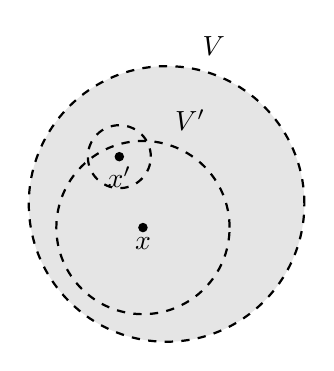
\begin{tikzpicture}
            \centering
            
            \def\radius{1.75}
            \def\incolor{gray!20}
    
            % Desactiva los caracteres conflictivos
            \shorthandoff{>} % Para poner puntas de flecha
    
            \filldraw[dashed, fill=\incolor, thick] (0,0) circle (\radius) node[above, yshift=\radius cm, xshift=0.6cm] {$V$};
            % \filldraw (0,0) circle (1.5pt)  node[below] {$x$};

            \def\radius{0.4}
            \draw[dashed, thick] (-0.6,0.6) circle (\radius);
            \filldraw (-0.6,0.6) circle (1.5pt)  node[below] {$x'$};

            \def\radius{1.1}
            \draw[dashed, thick] (-0.3,-0.3) circle (\radius) node[above, yshift=\radius cm, xshift=0.6cm] {$V'$};
            \filldraw (-0.3,-0.3) circle (1.5pt)  node[below] {$x$};

        \end{tikzpicture}
    \end{center}
    
    \begin{proof}\
        \begin{enumerate}
            \item[\apuntar{V4}] $V\in \cc{B}_x\subset \cc{N}_x$, entonces, por \apuntar{N5} $\exists N'\in \cc{N}_x$ con $N'\subset V$ tal que $V \in \cc{N}_y$\ \ $\forall y \in N'$. Como $\cc{B}_x$ es b.d.e, $\exists V'\in \cc{B}_x$ con $V'\subset N'\subset V$.\\
            
            Sea $y\in V'\subset N'\Rightarrow V\in \cc{N}_y$. Como $\cc{B}_y$ es b.d.e, $\exists V_y \in \cc{B}_y$ con $V_y \subset V$.
        \end{enumerate}
    \end{proof}
\end{prop}

\begin{prop}
    Sea $X \neq \emptyset$ un conjunto y supongamos que $\forall x \in X$ tenemos una familia $\cc{B}_x \subset \cc{P}(X)$ cumpliendo \apuntar{V1}, \dots, \apuntar{V4}. Entonces existe una única topología $\cc{T}$ en $X$ tal que $\cc{B}_x$ es b.d.e de $x$ en $(X,\cc{T})$\ \ $\forall x \in X$.\\

    Además, $\cc{T}$ es la única topología con $\cc{N}_x=\{N\subset X : \exists V=V_x \in \cc{B}_x\text{ con }V_x\subset N\}$\ \ $\forall x \in X$.

    \begin{proof}
        Tengo que comprobar que $\cc{N}_x$ cumplen \apuntar{N1},\dots, \apuntar{N5} usando que $\cc{B}_x$ cumplen \apuntar{V1}, \dots, \apuntar{V4}. La demostración se deja propuesta como ejercicio para el lector. % TODO
    \end{proof}
\end{prop}

\begin{ejercicio}
    Sean $(X, \cc{T})$ y $(X, \cc{T}')$ espacios topológicos y $\cc{B}_x$ b.d.e de $x$ en $(X,\cc{T})$\ \ $\forall x \in X$. Si $V$ es entorno de $x$ en $\cc{T}'$\ \ $\forall V \in \cc{B}_x$, entonces $\cc{T} \leq \cc{T}'$.ç
    \endsquare
\end{ejercicio}

\section{Puntos adherentes. Clausura}

\begin{definicion}
    Sean $(X, \cc{T})$ un e.t., $A\subset X$, $x\in X$. Diremos que $x$ es \textbf{adherente} de $A$ si $A\cap N\neq\emptyset$\ \ $\forall N \in \cc{N}_x$, es decir, si cada entorno del punto interseca al conjunto. Esto no implica que $x\in A$. Podemos distinguir dos tipos:
    \begin{itemize}
        \item Decimos que un punto adherente $x$ es de \textbf{acumulación} de $A$ si $A\cap(N\setminus\{x\})\neq \emptyset$\ \ $\forall N \in \cc{N}_x$ (Esto no implica que $x\in A$).
        \item Decimos que un punto adherente $x$ es \textbf{aislado} de $A$ si existe un entorno $N\in \cc{N}_x$ tal que $A\cap N=\{x\}$ (Esto sí implica que $x\in A$).
    \end{itemize}
    \endsquare
\end{definicion}

\begin{prop}
    Sea $(X, \cc{T})$ un e.t., $A\subset X, x \in X$. Equivalen:
    \begin{enumerate}
        \item[(i)] $x$ es adherente a $A$.
        \item[(ii)] $A\cap U \neq \emptyset$\ \ $f\forall U \in \cc{T}$ con $x\in U$.
        \item[(iii)] $\forall B \in \cc{B}$ con $x\in B$, donde $\cc{B}$ es base de $\cc{T}$.
        \item[(iv)] $A\cap V \neq \emptyset$\ \ $\forall V \in \cc{B}_x$ con $\cc{B}_x$ base de entornos de $x$.  
    \end{enumerate}

    \begin{proof}\
        \begin{itemize}
            \item[(iii) $\Rightarrow$ (iv)] Sea $V\in \cc{B}_x\Rightarrow \exists U \in \cc{T}$ con $x\in U \subset V$. Como $\cc{B}$ es base de $\cc{T}$, entonces $\exists B\in \cc{B}$ con $x\in B\subset U \subset V$. Por hipótesis, $B\cap A \neq \emptyset$, por lo que $V\cap A \neq \emptyset$
            \item[(iv)$\Rightarrow$(i)] Sea $N \in \cc{N}_x$. Como $\cc{B}_x$ es base de entornos de $x$, entonces $\exists V \in \cc{B}_x$ con $V\subset N$. Por hipótesis, $A\cap V\neq \emptyset \Rightarrow A\cap N \neq \emptyset$ por lo que $x$ es adherente a A.
        \end{itemize}
    \end{proof}
\end{prop}

\begin{observacion}
    Los puntos de acumulación y los puntos aislados admiten una caracterización análoga. %TODO
    \endsquare
\end{observacion}

\begin{definicion}
    Sea $(X, \cc{T})$, $A\subset X$. Se define la \textbf{adherencia} ( \textbf{clausura} o \textbf{cierre}) de $A$ como $\overline{A}=cl(A)=\{x\in X : x \text{ es adherente de } A\}$.
    \endsquare
\end{definicion}

\begin{ejemplo}\
    \begin{itemize}
        \item $\overline{\emptyset} = \emptyset$.
        \item $A\subset \overline{A}$. Para verlo puedo tomar $x\in A, N  \in \cc{N}_x$, entonces $x\in N\Rightarrow x \in N\cap A \neq \emptyset$ por lo que $x\in \overline{A}$.
        \item $\overline{X} = X$.
        \item Sea $(X,d)$ e.m. y tomamos $A\subset X, x \in X$. Entonces $x\in \overline{A}$ si $B(x,\veps)\cap A \neq \emptyset$\ \ $\forall \veps >0$.
    \end{itemize}
    \endsquare
\end{ejemplo}

\begin{ejemplo} En $(\bb{R}, \cc{T}_u)$
    \begin{itemize}
        \item $A=(0,1)\Rightarrow \overline{A}=[0,1]$ y todos los puntos son de acumulación.
        \item $A=(0,1)\cup \{2\}\Rightarrow [0,1]\cup\{2\}$. Además $x$ es de acumulación $\forall x \in [0,1]$ y $x=2$ es aislado (ya que puedo considerar $N=\left(\frac{3}{2}, \frac{5}{2}\right)\in \cc{N}_2$ y $N\cap A =\{2\}$).
    \end{itemize}
    \endsquare
\end{ejemplo}

\begin{prop}
    Sea $(X, \cc{T})$ un e.t y $A\subset X$. Entonces:
    \begin{enumerate}
        \item[(i)] $\overline{A}\in \cc{C}_{\cc{T}}$.
        \item[(ii)] Si $C\in \cc{C}_{\cc{T}}$ y $A\subset C$, entonces $\overline{A}\subset C$, es decir, la adherencia es el cerrado más pequeño que contiene a $A$. 
        \item[(iii)] $A=\overline{A}\sii A \in \cc{C}_{\cc{T}}$ .
    \end{enumerate}

    \begin{proof}\
        \begin{enumerate}
            \item[(i)] Supongamos que $\overline{A}=X$. Entonces $\overline{A}\in \cc{C}_{\cc{T}}$. Supongamos ahora el caso $\overline{A}\neq X\Rightarrow X\setminus \overline{A} \neq \emptyset$. Tendré que ver si $X\setminus \overline{A}\in \cc{T}$. Para ello tomo $x \in X\setminus \overline{A}$ y como $x\notin \overline{A}$, entonces $\exists U \in \cc{T}$ con $x\in U$, $U\cap A=\emptyset$, luego $U\cap \overline{A}=\emptyset$. Esto quiere decir que $x \in U\in X\setminus \overline{A}$ y entonces $X\setminus \overline{A} \in \cc{N}_x$\ \ $\forall x \in X\setminus \overline{A}$ por lo que $X\setminus \overline{A}\in \cc{T}$
            \item[(ii)] (Por reducción al absurdo) Supongamos $\overline{A}\cap (X\setminus C) \neq \emptyset$ y considero $x \in \overline{A}\cap (X\setminus C)$, entonces, como $(X\setminus C) \in \cc{T}$ tengo $x\in (X\setminus C) \in \cc{T}$ y como $x\in \overline{A}$, entonces $(X\setminus C)\cap A \neq \emptyset$, pero como teníamos que $A\subset C$ llegamos a contradicción
            \item[(iii)]
            \begin{itemize}
                \item[$\Rightarrow$)] $A=\overline{A} \overset{(i)}{\Rightarrow} A\in \cc{C}_{\cc{T}}$.
                \item[$\Leftarrow$)] Tengo que $A\in \cc{C}_{\cc{T}}$ y $A\subset A$ (trivialmente) $\overset{(ii)}{\Rightarrow} \overline{A}\subset A$ y como $A\subset \overline{A}$ (por lo visto anteriormente), se da la doble inclusión y tenemos que $A=\overline{A}$.
            \end{itemize} 
        \end{enumerate}
    \end{proof}
\end{prop}

\begin{ejemplo}(Ejercicio 23 de la Relación 1)
    \begin{enumerate}[label=\alph*)]
        \item $(X, \cc{T}_t)$, $A\subset X$, $\#A \geq 2 \Rightarrow \overline{A} = X$ ya que $X\cap A = A \neq \emptyset$\ \ $\forall x \in X$.
        \item $(X, \cc{T}_{disc})$, $A\subset X \Rightarrow \overline{A} = A$ ya que $A\in \cc{C}_{\cc{T}}$\ \ $\forall A \subset X$. Además, todos los puntos son aislados ya que $\forall x \in \overline{A}$\ \ $\exists \{x\}\in \cc{N}_x$, $A\cap \{x\} = \{x\}$.
        \item $(X, \cc{T}_{CF})$, $A\subset X$ infinito, entonces $\overline{A} = A$ (ya que al ser $A$ finito es cerrado). Además, todos los puntos serán aislados, ya que $\forall a \in A $ puedo considerar $U=(X\setminus A)\cup \{a\}\in \cc{N}_a$ y $U\cap A = \{a\}$.
        \item $(\bb{R}, \cc{T}_S)$ (una base de $\cc{T}_S$ es $\{[x, x+\veps ) : x \in \bb{R}, \veps>0\}$).
        
        $A=(0,1] \Rightarrow \overline{A} = [0,1]$. Además $x$ es de acumulación $\forall x \in[0,1)$ y $x=1$ es aislado.

        $A=(0,1) \Rightarrow \overline{A} = [0,1)$ (ya que puedo considerar $N=[1,2)\in \cc{N}_1$ y $N\cap A = \emptyset$ luego $1\notin \overline{A}$).
    \end{enumerate}
\end{ejemplo}

\begin{ejemplo}\
    \begin{itemize}
        \item $(\bb{R}^n , \cc{T}_u)$, $\overline{B(x,r)} = \overline{B}(x,r)$. Esto no es cierto en todo espacio métrico.
        \item $(\bb{R}, \cc{T}_u)$, $\overline{(a,b)} = [a,b] = \overline{(a,b]} = \overline{[a,b)}$. $\overline{\bb{Q}} = \bb{R} = \overline{\bb{R}\setminus \bb{Q}}$.
    \end{itemize}
    \endsquare
\end{ejemplo}

\begin{definicion}
    Sea $(X, \cc{T})$ un e.t., $A\subset X$, $A$ se dice \textbf{denso} si $\overline{A} = X$. El espacio $(X,\cc{T})$ se dice \textbf{separable} si $\exists A \subset X$ denso y numerable.
    \endsquare
\end{definicion}

\begin{ejemplo}\
    \begin{itemize}
        \item $(\bb{R}^n, \cc{T}_u)$ es separable $\overline{\bb{Q}}=\bb{R}^n$.
        \item $A\subset X$ denso $\sii A\cap B\neq \emptyset$\ \ $\forall B \in \cc{B}$ con $\cc{B}$ base de $\cc{T}$.
    \end{itemize}
\end{ejemplo}

\begin{prop}
    Sea $(X, \cc{T})$ un e.t., $A,B\subset X$. Entonces:
    \begin{enumerate}
        \item[(i)] $\overline{\overline{A}} = \overline{A}$.
        \item[(ii)] Si $A\subset B$, entonces $\overline{A}\subset \overline{B}$.
        \item[(iii)] $\overline{A\cup B} = \overline{A}\cup \overline{B}$.
        \item[(iv)] $\overline{A\cap B} \subset \overline{A}\cap \overline{B}$ (la otra inclusión no se verifica en general, por ejemplo, en $(\bb{R}, \cc{T}_u)$, los conjuntos $A=(0,1)$, $B=(1,2)$) 
    \end{enumerate}

    \begin{proof}\
        \begin{enumerate}
            \item[(i)] $\overline{A}\in \cc{C}_{\cc{T}}$ luego $\overline{\overline{A}} = \overline{A}$.
            \item[(ii)] $A\subset B \subset \overline{B}\in \cc{C}_{\cc{T}}\Rightarrow \overline{A}\subset \overline{B}$.
            \item[(iii)] 
            \begin{itemize}
                \item[$\subset$)] $A\cup B \subset \overline{A}\cup \overline{B}\in \cc{C}_{\cc{T}}\Rightarrow \overline{A\cup B}\subset \overline{A}\cup \overline{B}$.
                \item[$\supset$)]\ \\
                \vspace{-2cm}
                
                \begin{gather*}
                    \left.
                    \begin{array}{c}
                        A\subset A\cup B \subset \overline{A\cup B}\in \cc{C}_{\cc{T}} \Rightarrow \overline{A}\subset\overline{A\cup B} \\
                        B\subset A\cup B \subset \overline{A\cup B}\in \cc{C}_{\cc{T}} \Rightarrow \overline{B}\subset\overline{A\cup B}
                    \end{array}\right\} \Rightarrow \overline{A}\cup \overline{B}\subset \overline{A\cup B} \hspace*{5cm}
                \end{gather*}

            \end{itemize}
            \item[(iv)]\ \\
            \vspace{-2cm}

            \begin{gather*}
                \left.
                \begin{array}{c}
                    A\cap B \subset A \subset \overline{A}\in \cc{C}_{\cc{T}}\Rightarrow \overline{A\cap B}\subset \overline{A} \\
                    A\cap B \subset B \subset \overline{B}\in \cc{C}_{\cc{T}}\Rightarrow \overline{A\cap B}\subset \overline{B}
                \end{array}\right\} \Rightarrow \overline{A\cap B}\subset \overline{A}\cap \overline{B} \hspace*{5cm}
            \end{gather*}

        \end{enumerate}
    \end{proof}
\end{prop}

